\chapter{狭义相对论中的理想流体}
\label{chap4}
\section{流体}
\label{sec4.1}
在相对论性天体物理中,许多引力场源可以用理想流体作为一阶近似。一般而言,“流体(fluid)”是一种特殊的“\textbf{连续介质}(continuum)”,连续介质是大量粒子组成的系统,无法跟踪单个粒子的运动,而只能描述粒子集合的“平均”或者“集体”性质,例如单位体积的粒子数、能量密度、动量密度、压强、温度等等。湖水以及它产生的引力场不取决于单个水分子的状态,而只依赖于大量分子的平均性质。

然而,湖水的这种平均性质在各点可以不同:湖水底部的压强比上部更大,温度也随着深度变化。大气(也是流体)密度随位置的改变而改变。这产生了一个问题:应该取多少粒子的平均才合适。必须要取足够多的粒子,从而使得单个粒子的行为没有影响;但是也必须比较少,以保证相对均匀性:取平均的粒子的速度、动能与粒子间距等等不能相差太大。这种合适的取平均的粒子集合称为“\textbf{流体元 (element)}”。这是个不太精确但是很有用的概念,流体元包含大量粒子,它们的密度、平均速度、温度等等的取值可以视为相同。如果这种合适的集合不存在(例如\textbf{极度}稀薄的气体),则连续介质近似失效。

连续介质近似将所有体元赋予了相应的密度、温度等等物理量的值,由于这些体元被视为“很小的”,则这种近似在数学上意味着在\textbf{每一点}赋予了密度、温度等等的值。也就是说,连续介质是由在取值在每一时刻每一点的各种场来定义的。

连续介质的概念既包括岩石也包括气体。\textbf{流体}是“流动”的连续介质,这也是个不精确的定义,固体与流体的区别因而也不十分清楚。大多数固体在压强足够大时也会流动。什么让物体保持坚硬?是与两个体元界面\textbf{平行}的力。两个相邻体元可以互相挤压、拉伸,只有相邻体元不会沿分界面滑动的连续体才是刚性的。\textbf{流体}的特征是,那种阻碍滑动的力(沿平行于界面方向)远小于垂直于界面方向的力(称为压强)。\textbf{理想(perfect)流体}是\textbf{所有}阻碍滑动的力为零的流体,理想流体相邻体元之间的相互作用力只有压强。后面会用数学来精确描述这些性质。

\section{尘埃系统:数流密度向量$\vec{N}$}
\label{sec4.2}
本节以最简单“尘埃”系统为例引入描述流体的相对论性物理量。“尘埃 (dust)”系统由一组粒子组成,这些粒子在某个Lorentz坐标系中处于静止。我不知道这种系统为啥起名叫做灰尘(窗台上的东西),但是它是相对论的标准术语。

\subsection*{粒子数密度$n$}
对尘埃粒子最简单的问题是:单位体积内的粒子数是多少?在粒子静止的坐标系中,只需要数一数有多少粒子并除以体积就好了。由于系统各处的粒子疏密程度可能不同,因此不同点附近的小区域内的粒子数也会不同。定义\textbf{数密度 (number density)}\ $n$为:
\begin{equation}
    n := \text{流体元的MCRF观测到的数密度。}
\label{equ4.1}
\end{equation}
粒子在其中运动的坐标系$\MObar$观测到的数密度是什么?所有粒子在$\MObar$系中具有共同的速度$v$。同样的一组粒子在静止坐标系中和$\MObar$系观测的粒子数\textbf{相同},而占据的体积不同。设在静止坐标系,这组粒子占据长方形体积$\Delta x\, \Delta y\, \Delta z$,它在$\MObar$系中Lorentz收缩为$\Delta x\, \Delta y\, \Delta z \sqrt{1 - v^2}$,因为沿粒子运动的方向长度收缩而垂直方向长度不变(如图\ref{fig4.1})。因此,$\MObar$系的粒子数密度是静止系数密度乘以$(\sqrt{1 - v^2})^{-1}$:
\begin{equation}
    \frac{n}{\sqrt{1 - v^2}} = \Big\{\text{粒子在其中速度为$v$的坐标系 观测到的数密度} \Big\}.
\label{equ4.2}
\end{equation}

{
    \centering
    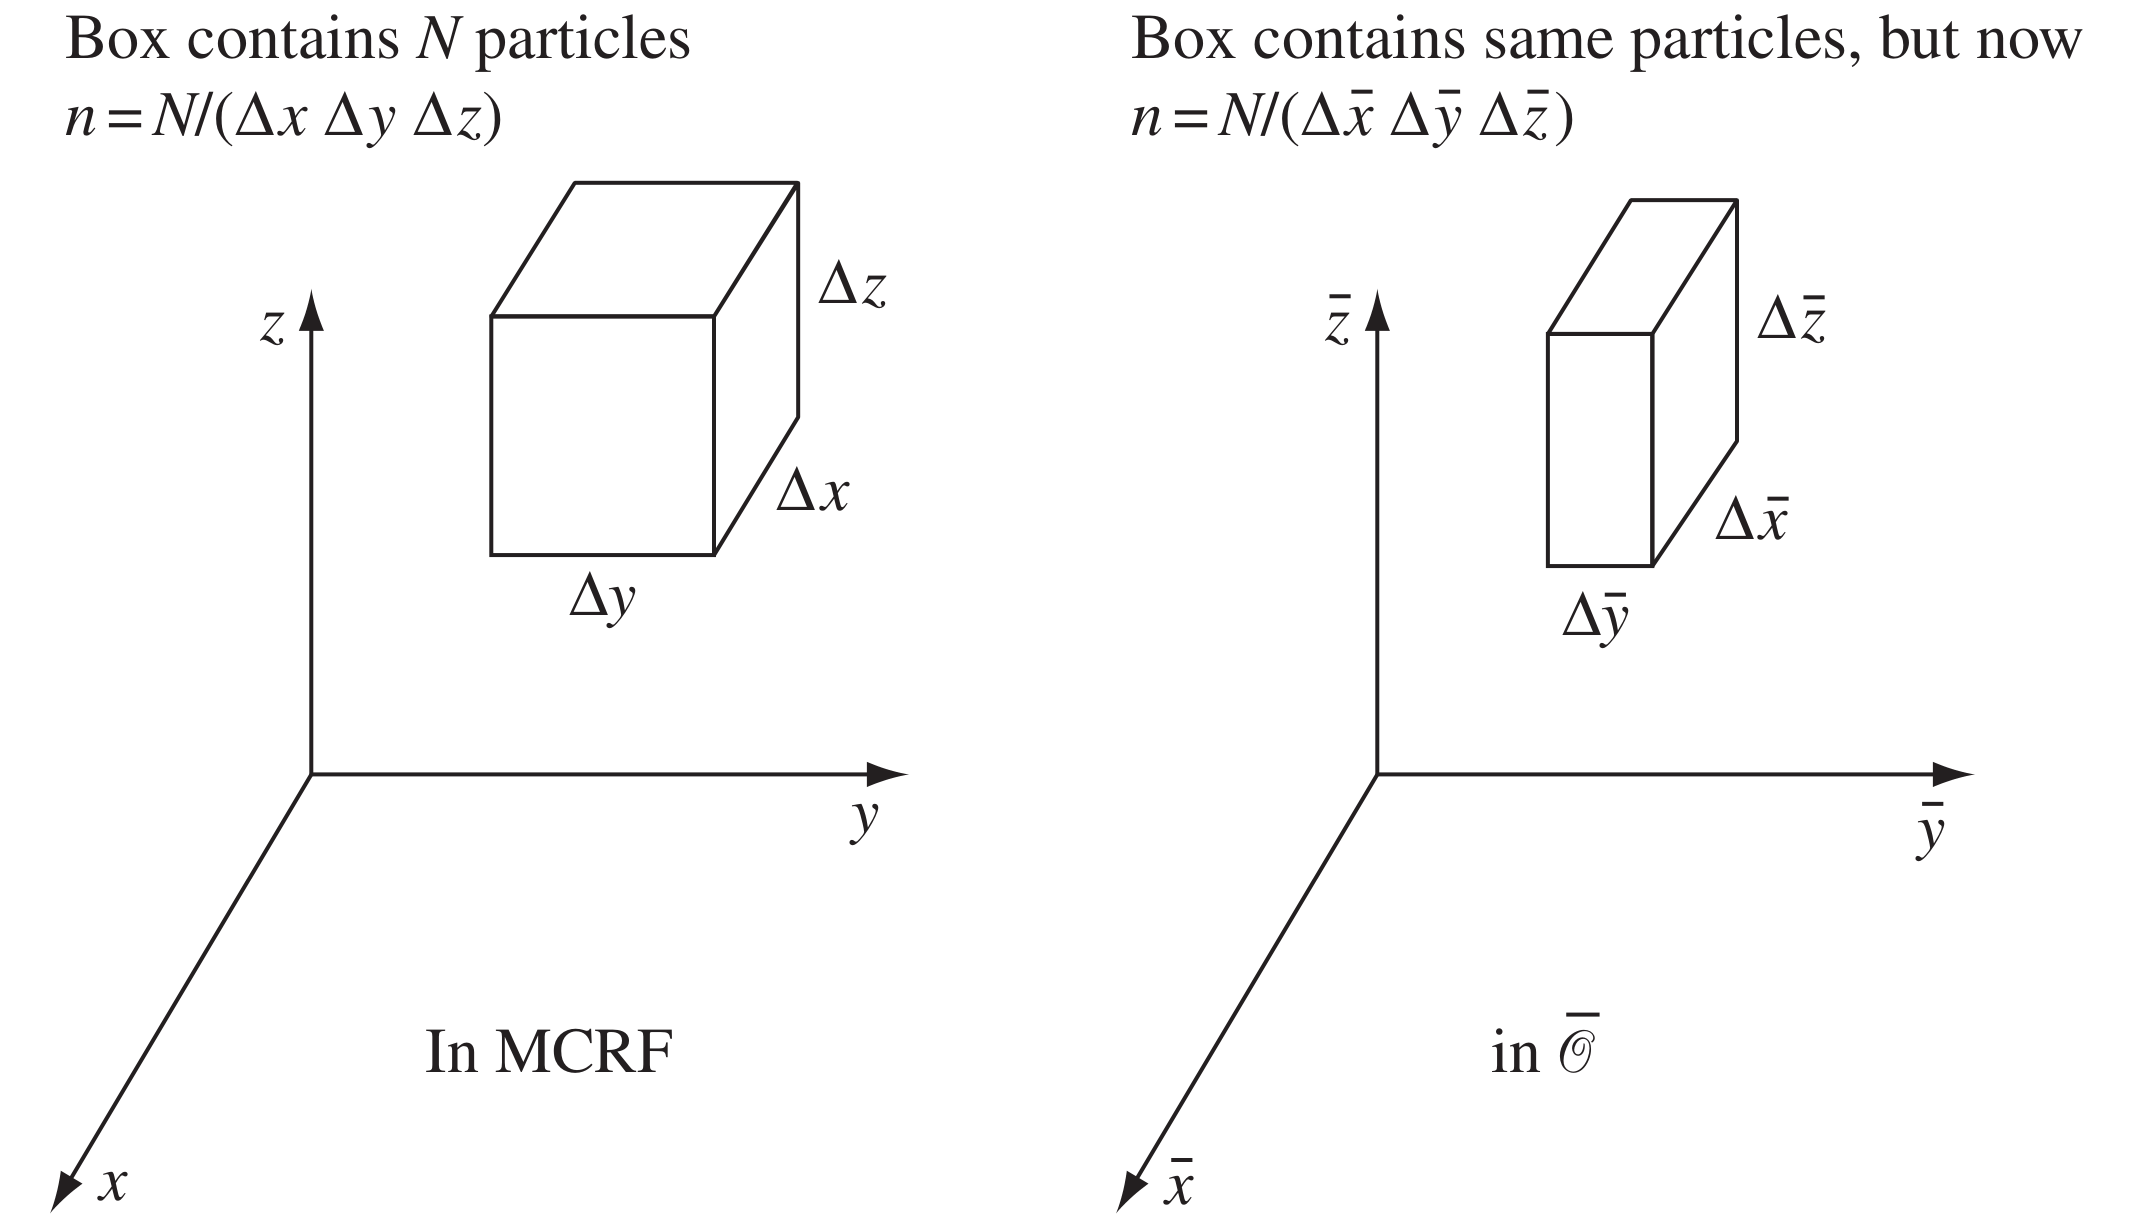
\includegraphics[width=0.7\textwidth]{fig4.1.png}
    \figcaption{\textit{Lorentz收缩使得粒子数密度依赖于坐标系。}}
    \label{fig4.1}
}

\subsection*{通过表面的流量}
对于运动的粒子,另一个有趣的问题是,沿某一方向“有多少”粒子运动?相应的精确概念是“流量(flux)”:\textit{粒子通过一个平面的流量是单位时间通过单位面积表面的粒子数}。显然,流量依赖于坐标系(“面积”与“时间”都依赖于坐标系)以及表面的方向(平行于粒子速度的表面,其流量为零,因为没有粒子通过它)。


{
    \centering
    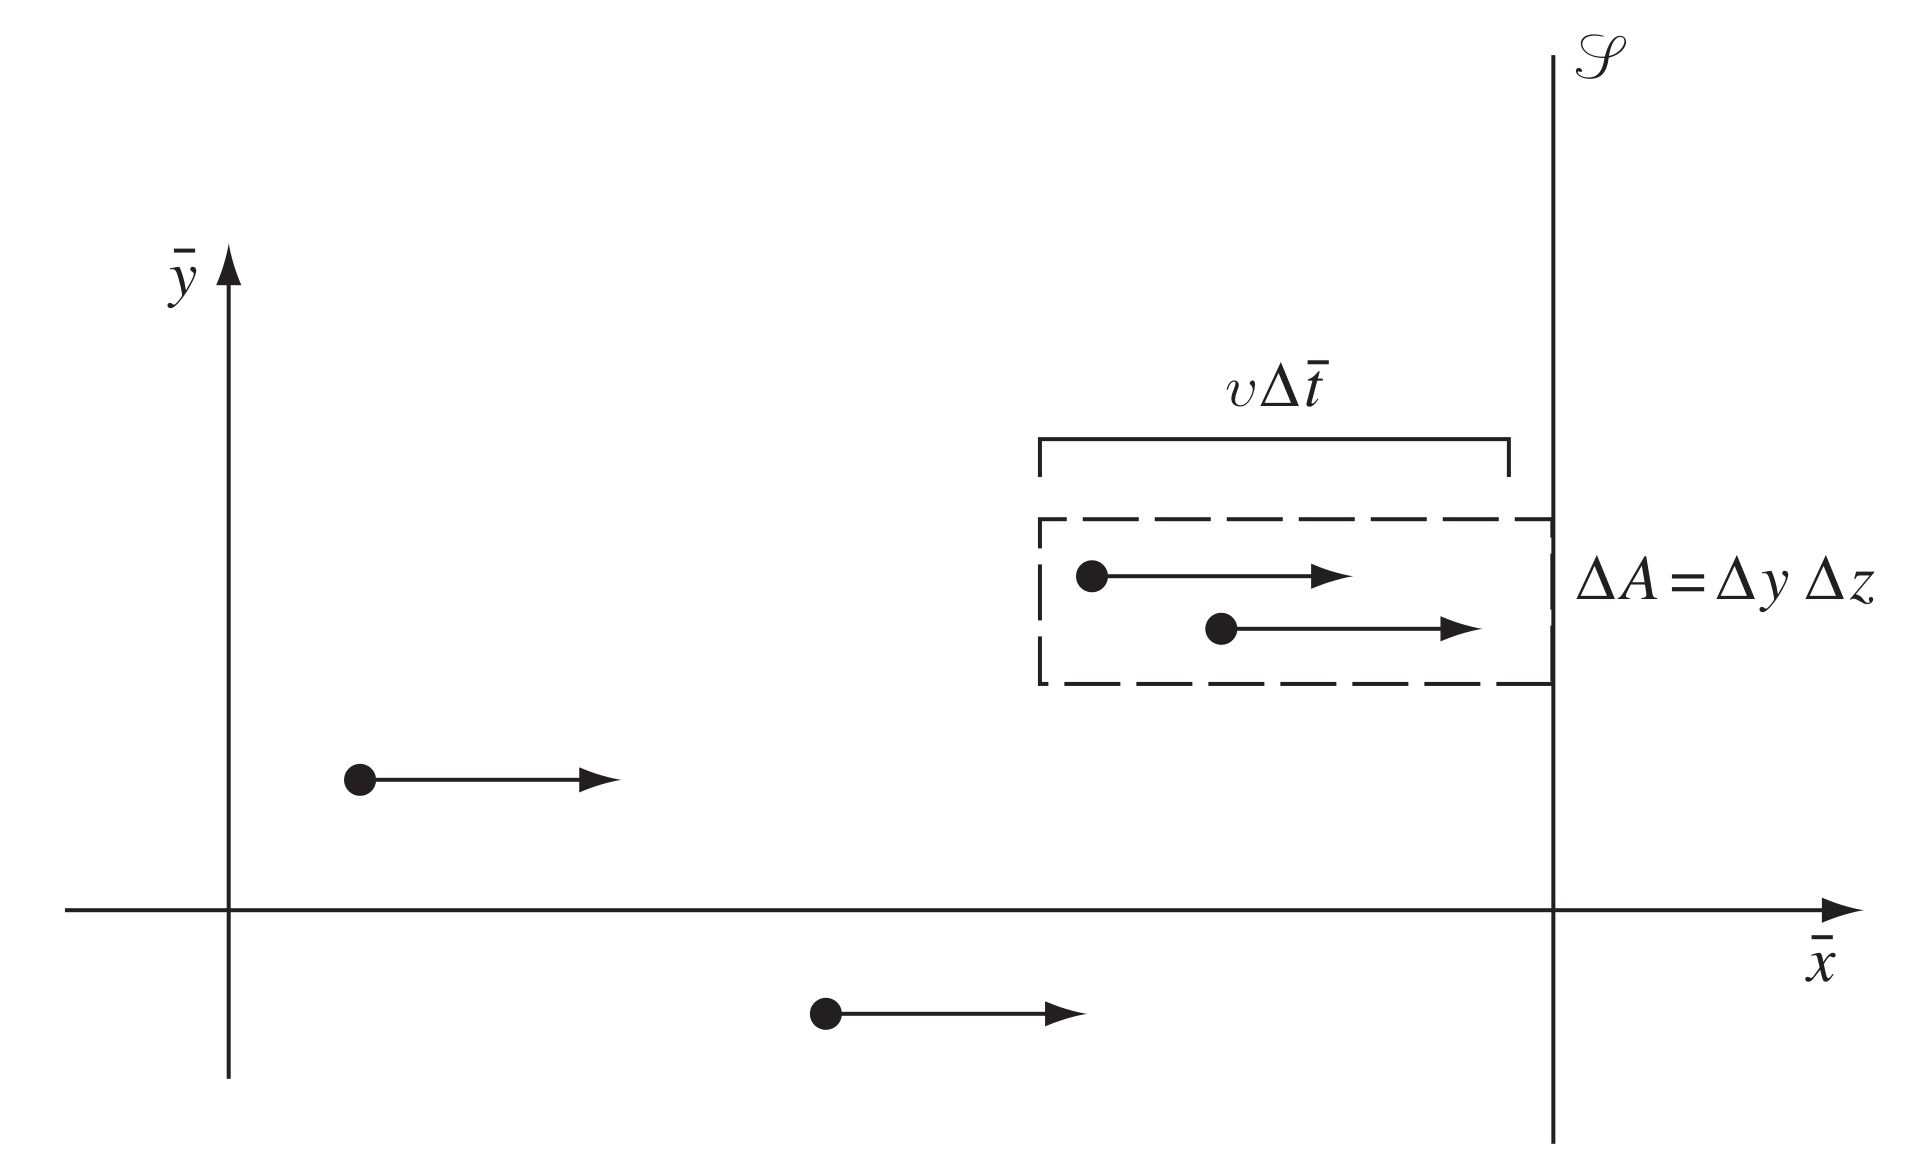
\includegraphics[width=0.7\textwidth]{fig4.2.png}
    \figcaption{\textit{流量变换律的简单图示:如果粒子只沿$x$轴运动,则在时间$\Delta \bar{t}$通过$\mathscr{S}$面的粒子位于距离$\mathscr{S}$面$v \Delta\bar{t}$的范围内。 }}
    \label{fig4.2}
}


在尘埃系统的静止坐标系中流量为零,因为所有粒子静止。设在$\MObar$系,所有粒子沿$\bar{x}$ 方向以速度$v$运动,先考虑垂直于$\bar{x}$轴的平面(如图\ref{fig4.2}),图中由虚线表示的立方体区域内的粒子就是在时间$\Delta \bar{t}$内通过$\mathscr{S}$面的面积$\Delta A$的粒子。这个区域的体积是$v \Delta \bar{t}\, \Delta A$,由于该系的数密度为$n / \sqrt{1 - v^2}$,因此该区域的粒子数为$[n / \sqrt{1 - v^2}] v \Delta \bar{t}$。\textbf{单位时间}内穿过等$\bar{x}$面($\mathscr{S}$面)单位面积的粒子数,也就是通过等$\bar{x}$面的流量为:

\[
    (\text{flux})^{\bar{x}} = \frac{nv}{\sqrt{1 - v^2}}.
\]

更一般的情况是,粒子在$\MObar$系中也有$\bar{y}$方向的速度,图\ref{fig4.3}中,在$\Delta \bar{t}$时间内通过$\mathscr{S}$面的面积$\Delta A$的粒子位于虚线区域内,该区域是“平行六面体”形状的,它的体积等于底乘以高,它的高——$\bar{x}$方向的长度——等于$v^{\bar{x}} \,\Delta \bar{t}$,由此可得

\begin{equation}
    (\text{flux})^{\bar{x}} = \frac{n v^{\bar{x}}}{\sqrt{1 - v^2}}.
\label{equ4.3}
\end{equation}

{
    \centering
    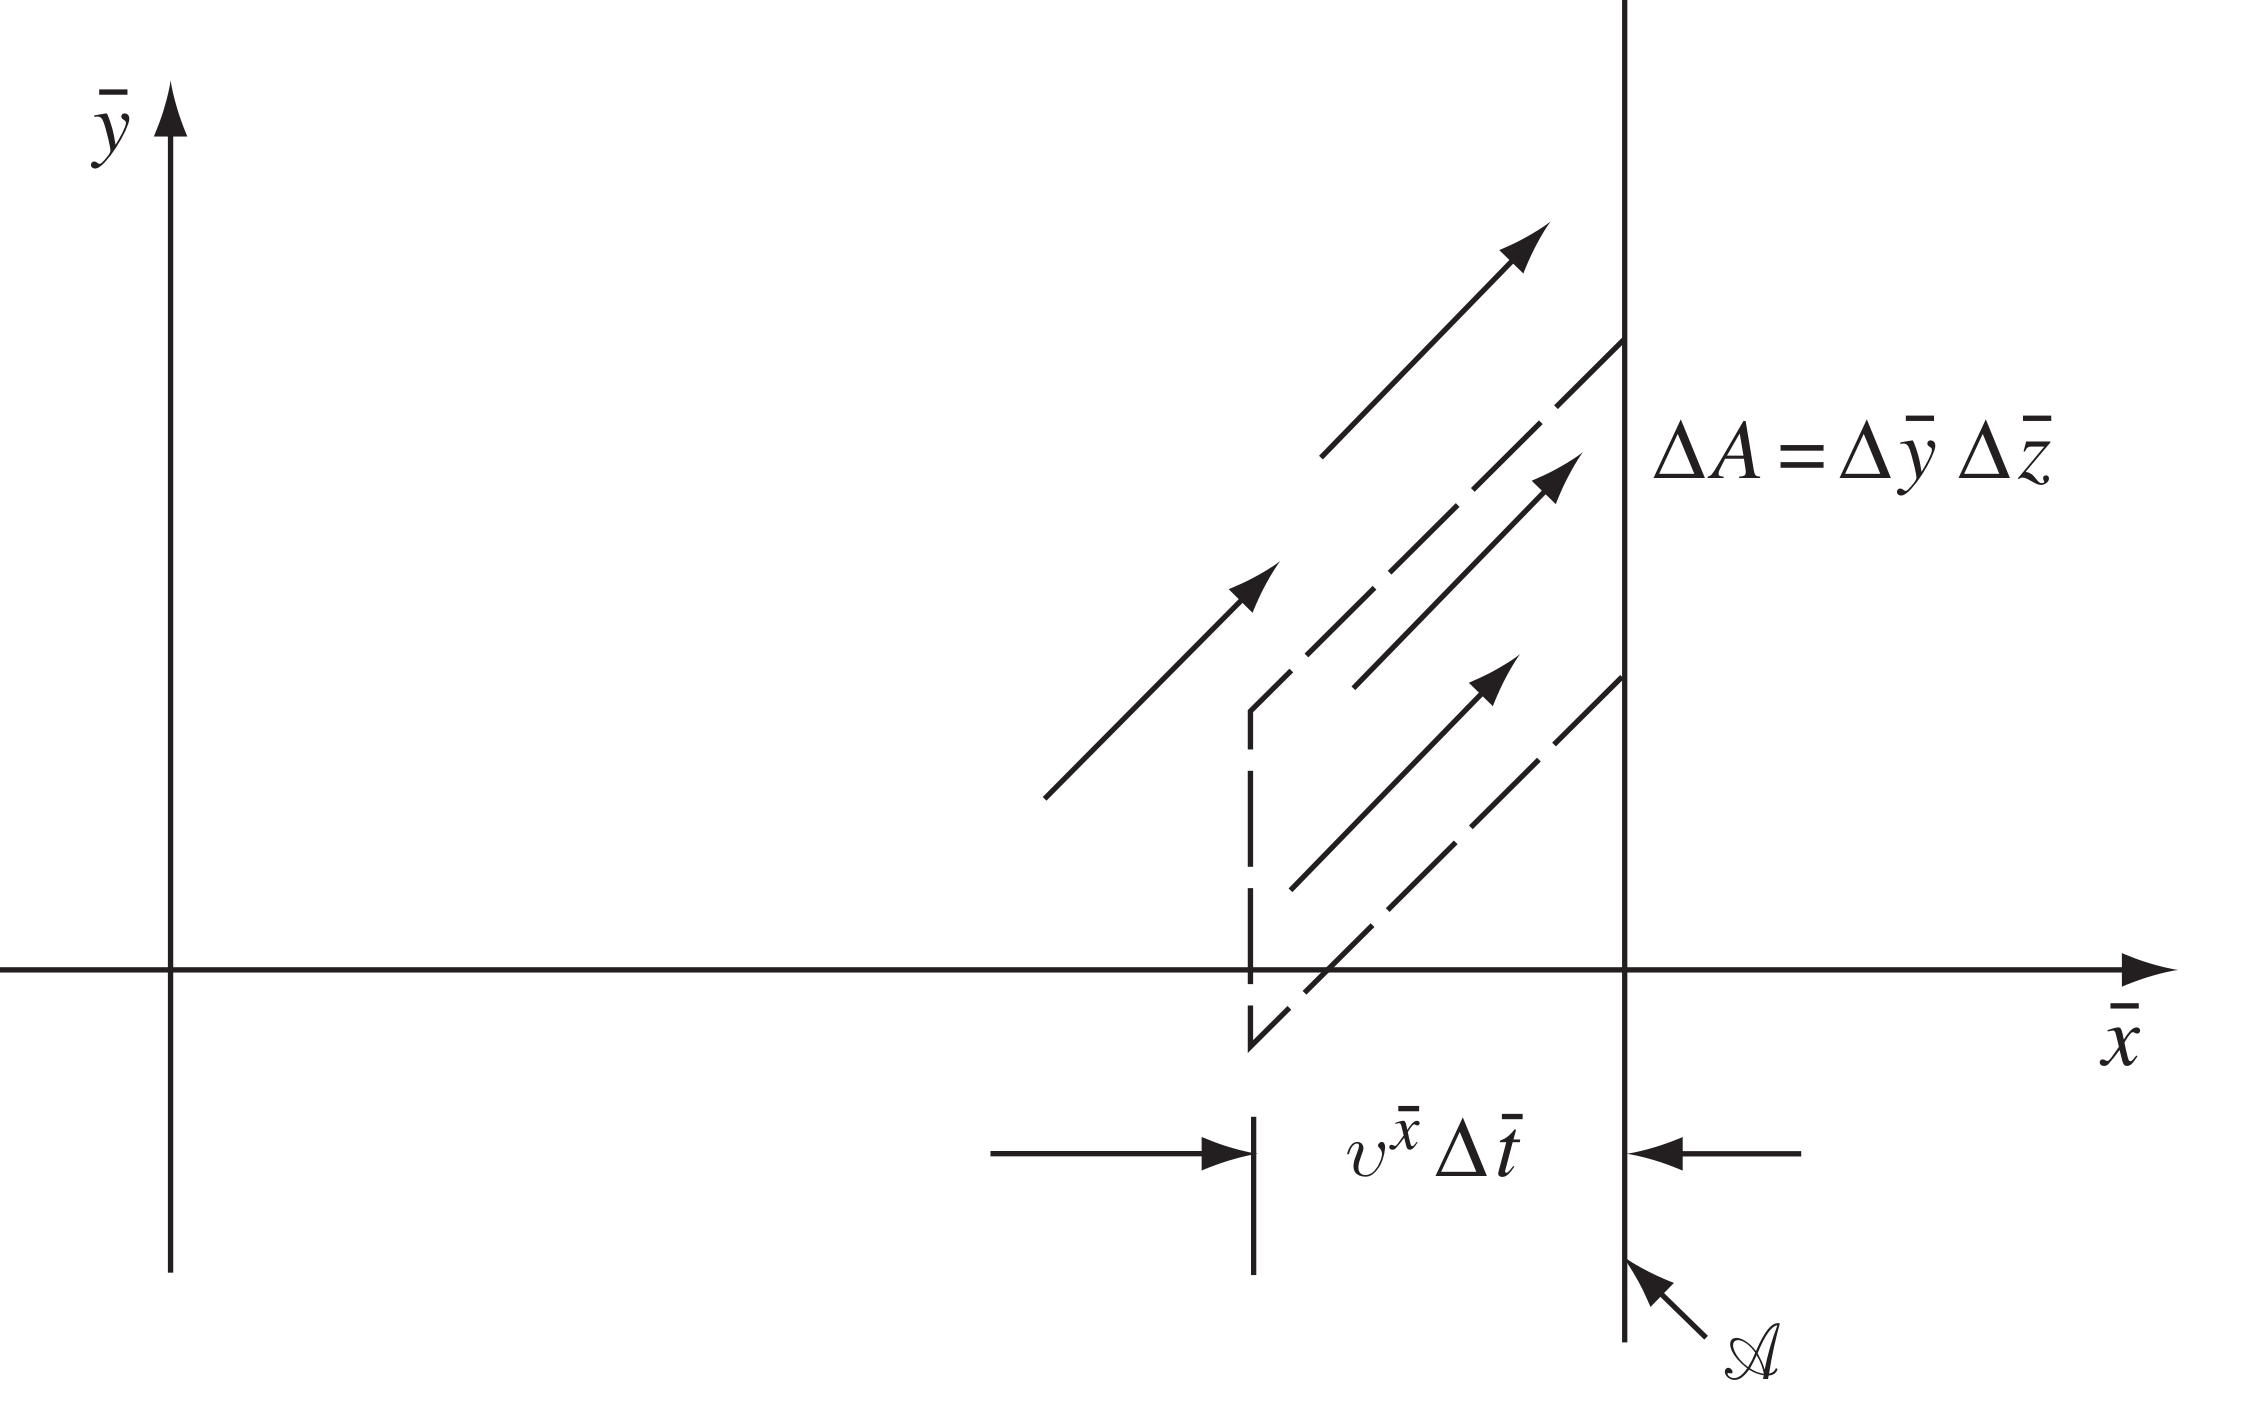
\includegraphics[width=0.7\textwidth]{fig4.3.png}
    \figcaption{\textit{流量的更一般情况:通过等$\bar{x}$坐标面的流量只与粒子速度的$\bar{x}$分量有关。}}
    \label{fig4.3}
}


\subsection*{数流密度四维向量$\vec{N}$}
定义向量$\vec{N}$为
\begin{shaded}
\begin{equation}
    \vec{N} = n \vec{U},
\label{equ4.4}
\end{equation}
\end{shaded}
其中$\vec{U}$是粒子四速。设在$\MObar$系中粒子速度为$(v^x, v^y, v^z)$,则有
\[
    \vec{U} \xrightarrow[\MObar]{ } \left( \frac{1}{\sqrt{1 - v^2}}, \frac{v^x}{\sqrt{1 - v^2}}, \frac{v^y}{\sqrt{1 - v^2}}, \frac{v^z}{\sqrt{1 - v^2}} \right).
\]
因此
\begin{equation}
    \vec{N} \xrightarrow[\MObar]{ } \left( \frac{n}{\sqrt{1 - v^2}}, \frac{nv^x}{\sqrt{1 - v^2}}, \frac{n v^y}{\sqrt{1 - v^2}}, \frac{n v^z}{\sqrt{1 - v^2}} \right).
\label{equ4.5}
\end{equation}
可见,在任意坐标系中,$\vec{N}$的时间分量是数密度,空间分量是通过不同坐标面的流量。这个概念超级重要。在伽利略的物理学中,数密度是个在所有坐标系都相同的标量(没有Lorentz收缩),而流量是很不一样的物理量:它是\textbf{依赖于}坐标系的三维向量,因为粒子速度依赖于坐标系。在相对论中,数密度与流量被统一到同一个不依赖于坐标系的四维向量当中。这是思维方式最主要的一大进步:将看起来无关的概念统一到一个量。

值得再次强调“不依赖于坐标系”的含义。向量$\vec{N}$是个几何量,它的存在不依赖于任何坐标系;就像一般的张量那样,$\vec{N}$将1形式映射为数字,与坐标系无关。它的分量\textbf{确实}依赖于坐标系。由于相对论之前的物理学认为流量是三维向量,并且还依赖于坐标系:流量是三维向量,因为它与坐标轴的指向无关(就像四维向量与坐标系无关那样);但是流量这种三维向量在相互运动的坐标系中的分量不同,因为粒子的速度在这些坐标系中不同。对于旧物理学,流量向量必须在某个惯性系定义。而相对论只需要定义\textbf{一个}向量,旧物理学中坐标依赖的定义方式是因为只考虑了$\vec{N}$的四个分量中的三个。伽利略物理学中的坐标系无关量——数密度,和依赖于坐标系的量——流量,在相对论中被统一到了一个不依赖坐标系的四维向量$\vec{N}$当中,就像“能量”和“动量”被统一到了四维动量中那样。

最后,根据定义显然有
\begin{shaded}
\begin{equation}
    \vec{N} \cdot \vec{N} = -n^2, \quad n = (- \vec{N} \cdot \vec{N})^{1/2}.
\label{equ4.6}
\end{equation}
\end{shaded}
可见$n$是个标量。就像“静质量”是标量,而能量与“惯性质量”依赖于坐标系那样,“静密度”(静止坐标系观测到的粒子数密度)$n$是标量,而“数密度”依赖于坐标系。$n$\textbf{总是}定义为粒子的MCRF观测到的数密度,也就是一个标量。流体的压强、温度等其它特征量的定义也是如此,之后会讨论它们。

\section{1形式与表面}
\label{sec4.3}

\subsection*{数密度是一种类时流量}
为了进一步完善上面数密度与流量的统一,我们来论证数密度可以视为一种类时流量(timelike flux)。还是先考虑通过等$\bar{x}$坐标面的流量,在\textbf{时空图}中画出相应过程,如图\ref{fig4.4},图中只画出了$\bar{t}$轴和$\bar{x}$轴。

{
    \centering
    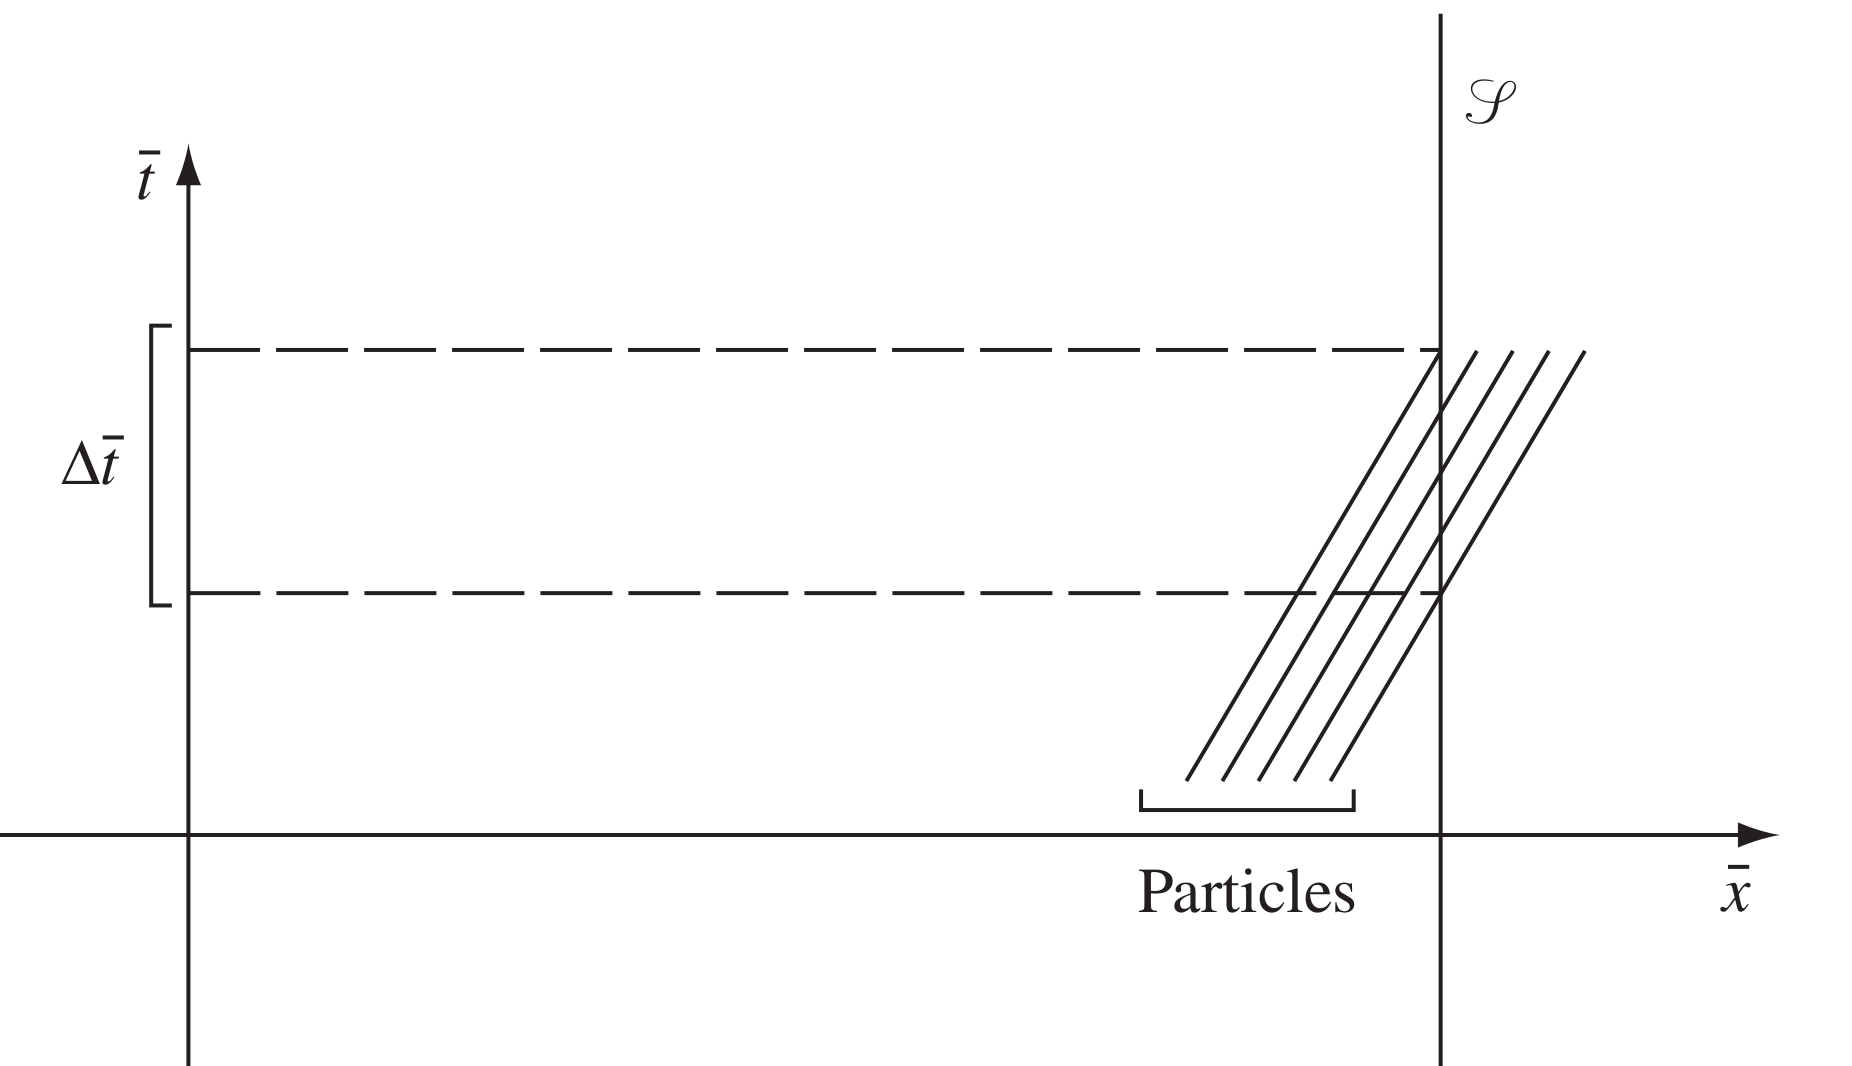
\includegraphics[width=0.7\textwidth]{fig4.4.png}
    \figcaption{\textit{图\ref{fig4.2}的时空图版本,其中省略了$\bar{y}$轴。}}
    \label{fig4.4}
}

垂直于$\bar{x}$轴的$\mathscr{S}$面的世界线如图所示,由于省略了$\bar{y}, \bar{z}$轴,因此任意时刻$\bar{t}$只对应一个点。在时间$\Delta \bar{t}$内通过$\mathscr{S}$面的粒子的世界线是图中的倾斜直线,流量即为在时间间隔$\Delta \bar{t} = 1$之内穿过$\mathscr{S}$面的粒子世界线数目。实际上,由于$\mathscr{S}$面是二维的,因此它的“世界轨迹”是三维的(“世界体”),而图中只能画出一部分。\textbf{流量}是通过单位“体积”世界体的世界线数目:单位体积的含义是边长为1单位的立方体$\Delta \bar{t} = 1, \Delta \bar{y} = 1, \Delta \bar{z} = 1$。因此,流量可以定义为通过三维世界体单位体积的粒子世界线数目。同理,这种三维世界体也可以是某一时刻$\bar{t}$对应的三维空间体的单位体积$\Delta \bar{x} = 1, \Delta \bar{y} = 1, \Delta \bar{z} = 1$,如图\ref{fig4.5}。这样,流量就是通过$\Delta \bar{x} = 1$($\Delta \bar{y}, \Delta \bar{z}$省略了)的世界线数目,而它正是特定时刻的单位体积内的粒子数:数密度。因此“类时”流量是数密度。

{
    \centering
    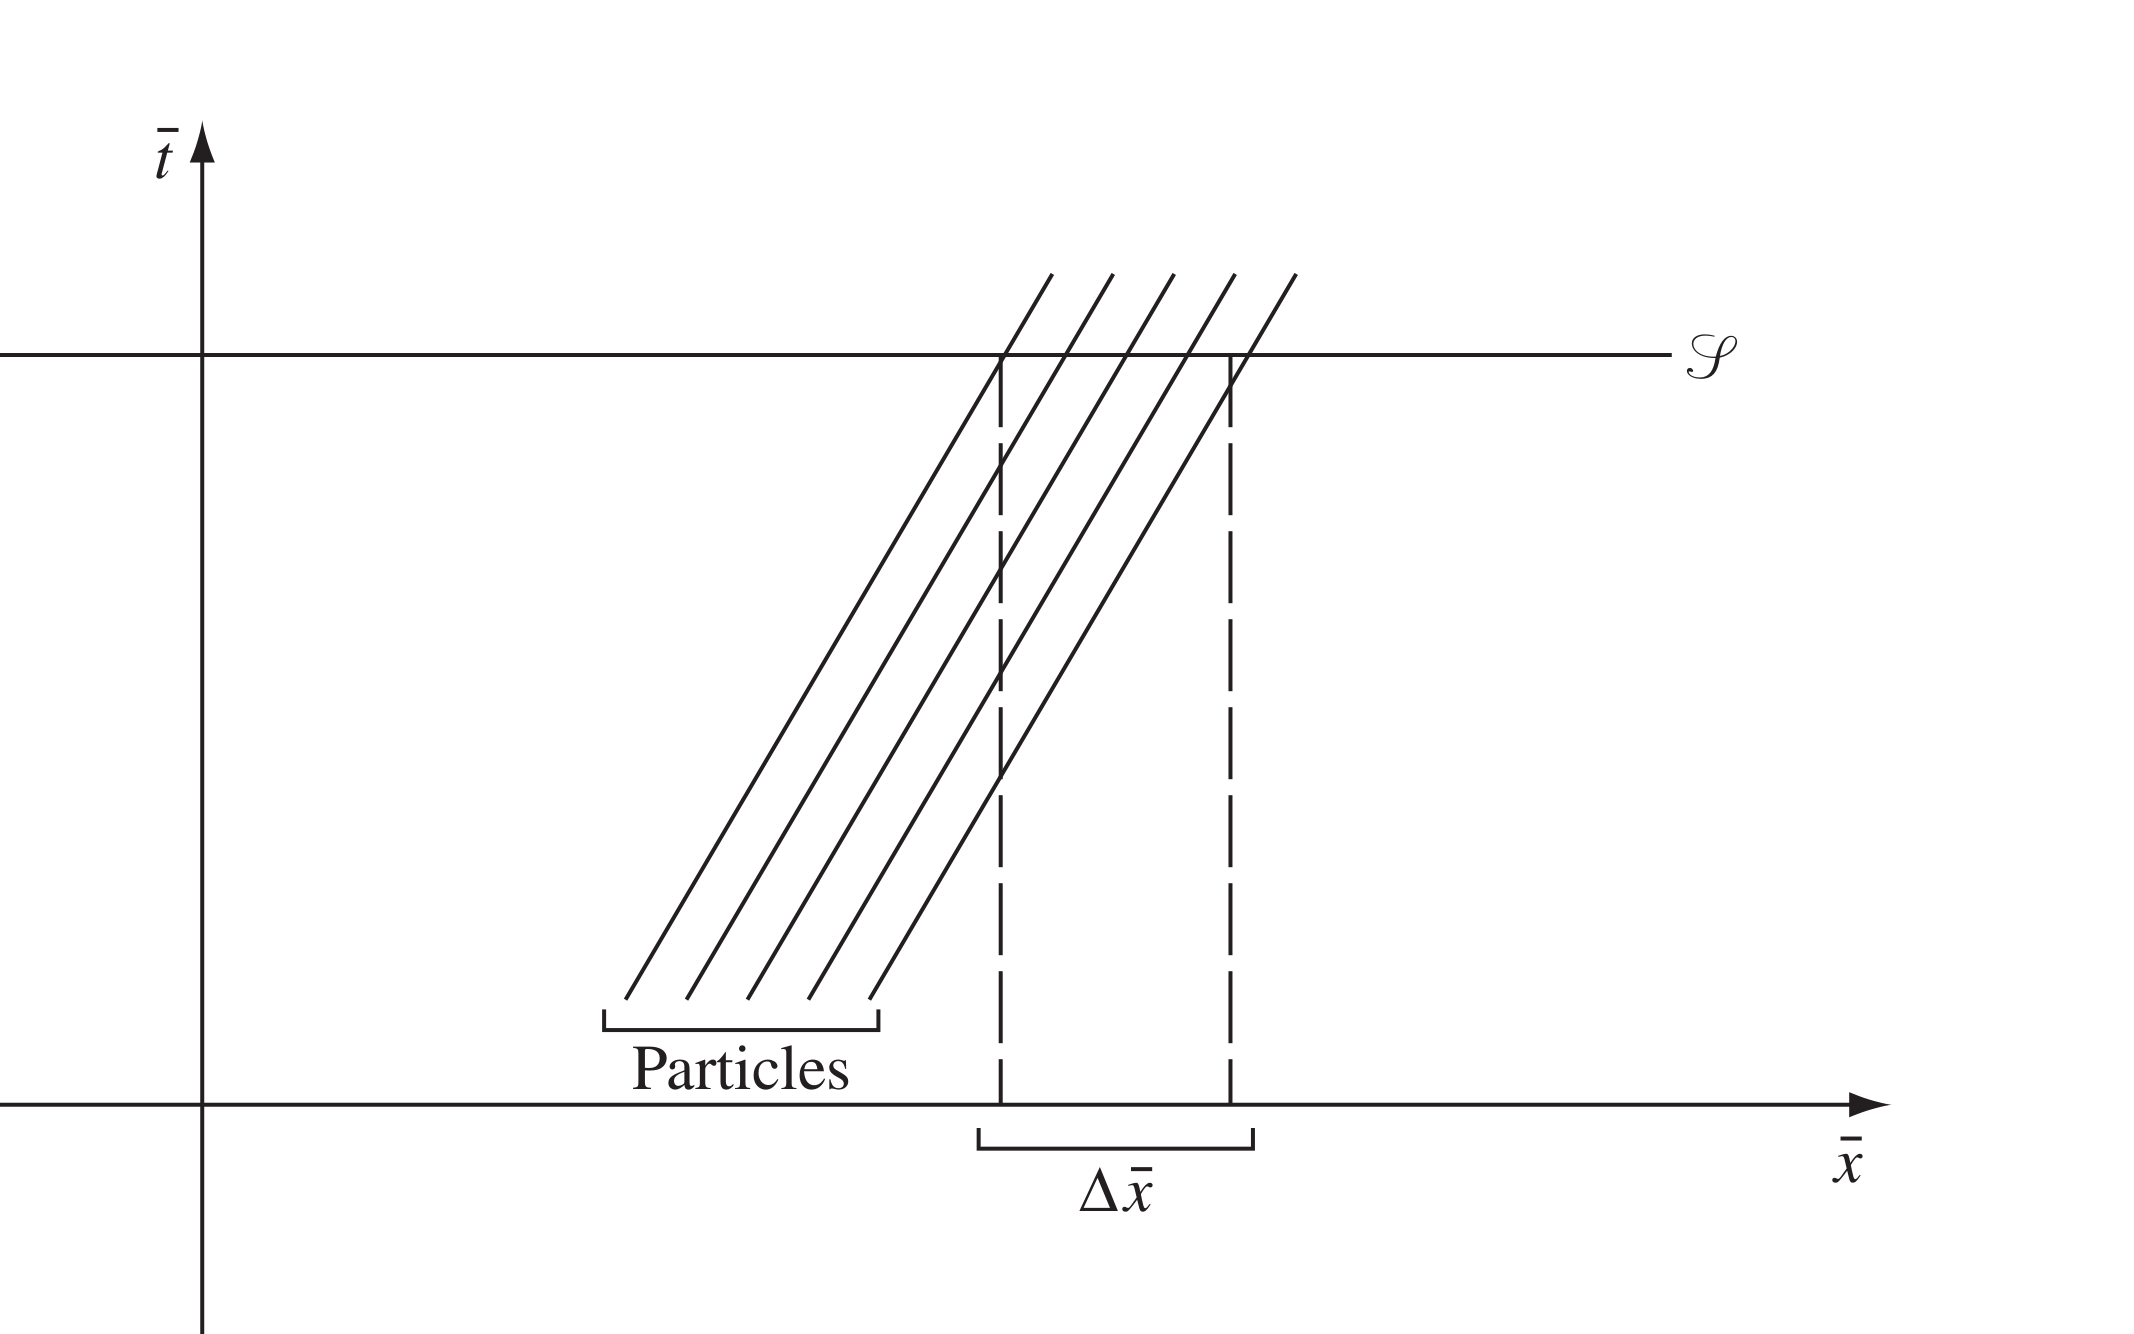
\includegraphics[width=0.7\textwidth]{fig4.5.png}
    \figcaption{\textit{数密度可以视为通过等时面$\bar{t} = \text{常数}$\ 的流量。}}
    \label{fig4.5}
}

\subsection*{一个1形式定义了一个表面}
前文描述表面的方式有点笨拙。为了用更加具有不变性的方式描述,需要用一种数学概念来表示粒子世界线所通过的表面,这要用到1形式。一般地,一个表面是由某个方程的解定义的:
\[
    \phi(t, x, y, z) = \text{常数。}
\]
函数$\phi$的梯度$\trd \phi$是法向1形式。某种程度上,$\trd \phi$\textbf{定义了}表面$\phi = \text{常数}$,因为它唯一确定了表面的法方向。然而,$\trd \phi$的任意常数倍也定义了同样的表面,因此一般采用单位法向1形式(unit-normal one-form)来描述not null的表面:
\begin{equation}
    \tilde{n} := \frac{\trd \phi}{|\trd \phi|},
\label{equ4.7}
\end{equation}
其中
\begin{align}
    |\trd \phi| \text{是}\trd\phi \text{的模:}\quad |\trd \phi| = |\eta^{\alpha \beta} \phi_{, \alpha} \phi_{, \beta} |^{1/2}. \label{equ4.8}
\end{align}
(不要把$\tilde{n}$和$n$混淆,后者是MCRF观测到的数密度,两者截然不同,只是由于偶然的历史原因使得它们的字母相同。)

就像三维空间的向量分析(例如高斯定律)那样,定义“面元(surface element)”为单位法向1形式乘以表面面元的面积。这样,坐标为$x^\alpha, x^\beta, x^\gamma$($\alpha, \beta, \gamma$是\textbf{特定的}、互不相同的指标)的三维体积元可以表示为
\begin{equation}
    \tilde{n} \rd x^\alpha \, \rd x^\beta \, \rd x^\gamma,
\label{equ4.9}
\end{equation}
而\textbf{单位}体积元($\rd x^\alpha = \rd x^\beta = \rd x^\gamma = 1$)就是$\tilde{n}$。(这些$\rd x$是要被积分掉的无穷小量,而非梯度。)

\subsection*{通过表面的流量}
回顾一下三维空间的高斯定律,它表明通过表面的流量,例如电场通量为$\bm{E} \cdot \bm{n}$,即电场$\bm{E}$与单位法向量的点乘。这里的情况也差不多:(粒子)通过等$\phi$面的流量是$\langle \tilde{n}, \vec{N} \rangle$。为了证明该式,先考虑$\phi$是坐标之一,例如$\bar{x}$的情况。等$\bar{x}$面的法向1形式为$\trd \bar{x}$,它也是单位1形式,因为$\trd \bar{x} \xrightarrow[\MObar]{ } (0, 1, 0, 0)$。则$\langle \trd \bar{x}, \vec{N} \rangle = N^\alpha (\trd \bar{x})_\alpha = N^{\bar{x}}$,由上文可见这就是通过$\bar{x}$坐标面的流量。显然,如果选择$\phi = \bar{t}$,则$\langle \trd \bar{x}, \vec{N} \rangle$的结果为$N^{\bar{0}}$——数密度,亦即通过等$\bar{t}$面的流量。

向量的定义是把1形式映射为实数的函数,上面是该定义的第一个物理实例。给定向量$\vec{N}$,可以计算通过某个面的流量——将向量与该平面的单位法向1形式缩并即可。此外,这个不依赖于坐标系的表达式$\langle \trd \bar{x}, \vec{N} \rangle$还把粒子系统的性质$\vec{N}$与表面的性质$\tilde{n}$分离开来。在下面的\ref{sec4.4}节还会讨论类似内容。

\subsection*{用1形式表示坐标系}
在继续讨论流体的其它性质之前,我们应该介绍一个有用的结论。目前我们用四维速度来定义一个惯性系,它也可以用1形式定义,也就是用四维速度对应的1形式$\mathbf{g} (\vec{U}, \ )$,它的分量为
\[
    U_\alpha = \eta_{\alpha \beta} U^\beta,
\]
在它所表示的坐标系中:
\[
    U_0 = -1, \quad U_i = 0.
\]
显然这个1形式等于$-\trd \bar{t}$(它们的分量相等)。由此可见,给定一个$\trd t$就等效地定义了一个惯性坐标系。相应的物理图像是:$\trd t$可以视为一组等$t$面,在同一个表面上的时刻相等。这显然定义了一个坐标系,只是还有一些空间坐标旋转的自由度(通常可以忽略)。实际上,$\trd t$某种程度上比$\vec{U}$的定义更加自然。例如,四动量为$\vec{p}$的粒子在$\trd t$表示的坐标系中的能量为
\begin{equation}
    E = \langle \trd t, \vec{p} \rangle = p^0.
\label{equ4.10}
\end{equation}
这样不会出现方程\eqref{equ2.35}当中不方便的负号:
\[
    E = -\vec{p} \cdot \vec{U}.
\]

\section{还是尘埃系统:应力-能量张量}
\label{sec4.4}
目前我们讨论了如何描述尘埃系统的粒子数,粒子也有能量、动量,后面会看到,它们的能量动量是GR中的引力场源。因此需要研究如何用具有坐标系不变性的方式描述这些量。简明起见,假设所有尘埃粒子具有相同的静质量$m$。

\subsection*{能量密度}
在MCRF中,每个粒子的能量为$m$,单位体积的粒子数为$n$,因此单位体积的能量为$mn$,将它记作$\rho$:
\begin{equation}
    \rho := \text{MCRF观测到的能量密度。}
\label{equ4.11}
\end{equation}
$\rho$是标量,就像$n, m$那样。对于尘埃系统:
\begin{equation}
    \rho = nm \text{(尘埃系统)。}
\label{equ4.12}
\end{equation}
对于更一般的流体,需要考虑粒子的随机热运动动能,即使在所有粒子的平均速度为零的坐标系内,\eqref{equ4.12}式也不再有效。

$\MObar$系观测到的数密度为$n / \sqrt{1 - v^2}$,由于所有粒子在$\MObar$系速度为$v$,因此粒子在该系的能量为$m / \sqrt{1 - v^2}$。因此能量密度为$mn / \sqrt{1 - v^2}$:
\begin{equation}
    \frac{\rho}{1 - v^2} = \Big\{ \text{粒子在其中的速度为$\bm{v}$的坐标系观测到的能量密度。} \Big\}.
\label{equ4.13}
\end{equation}
这个变换式含有两个因子$(1 - v^2)^{-1/2} = \Lambda\indices{^{\bar{0}}_0}$,因为体积与能量\textbf{二者都}进行了变换。因此能量密度不可能是某个向量的分量,实际上它是某个$\binom{2}{0}$张量的分量。这可以通过张量的定义看出。定义能量需要一个1形式,从而得到四动量的0分量;定义密度也需要一个1形式,因为密度是通过某个等时面的流量。于是,定义能量流量(简称为“能流”)需要两个1形式:1个定义能量、1个定义表面。同理,定义动量密度(momentum density)需要两个1形式:1个定义动量分量、1个定义密度。动量流(momentum flux)(定义为动量(的某个分量)通过某个表面的速率)也一样需要两个1形式。这些量可以统一为一个$\binom{2}{0}$张量$\textbf{T}$,其名为\textbf{应力-能量张量}(stress-energy tensor),这个张量将两个合适的1形式映射为相应的值。

\subsection*{应力-能量张量}
应力-能量张量最方便的定义是在某个(任意)坐标系中给出它的分量:

\begin{shaded}
\begin{equation}
    \mathbf{T} (\trd x^\alpha, \trd x^\beta) = T^{\alpha \beta} := \Bigg\{ \text{$\alpha$动量通过等$x^\beta$面的流量} \Bigg\}.
\label{equ4.14}
\end{equation}
\end{shaded}
(其中$\alpha$动量是指四动量的$\alpha$分量:$p^\alpha := \langle \trd x^\alpha, \vec{p} \rangle$。)上式符合张量的定义,证明作为本章习题5。

下面来讨论这个定义是怎样符合上文内容的。

\begin{itemize}
    \item $T^{00}$定义为0动量(能量)通过等时面$t = \text{constant}$\ 的流量,也就是能量密度:
    \begin{equation}
        T^{00} = \text{能量密度。}
    \label{equ4.15}
    \end{equation}
    \item $T^{0i}$是能量通过坐标面$x^i$(即表面$x^i = \text{常数}$)的流量:
    \begin{equation}
        T^{0i} = \text{通过$x^i$坐标面的能量流。}
    \label{equ4.16}
    \end{equation}
    \item $T^{i0}$是$i$动量通过$t = \text{constant}$\ 面的流量,也就是$i$动量密度:
    \begin{equation}
        T^{i0} = \text{$i$动量密度。}
    \label{equ4.17}
    \end{equation}
    \item $T^{ij}$是$i$动量的$j$流量:
    \begin{equation}
        T^{ij} = \text{通过$x^j$坐标面的$i$动量流量。}
    \label{equ4.18}
    \end{equation}
\end{itemize}
只要给定了$\mathbf{T}$在任意坐标系的分量,则它在其余坐标系的分量随之确定。对于尘埃系统,$\mathbf{T}$在MCRF的分量非常简单,在MCRF中的尘埃粒子速度为零,因此所有的$i$动量为零、空间流量为零,于是:
\begin{align*}
    (T^{00})_{\text{MCRF}} &= \rho = mn, \\
    (T^{0i})_{\text{MCRF}} &= (T^{i0})_{\text{MCRF}} = (T^{ij})_{\text{MCRF}} = 0.
\end{align*}
容易验证,张量$\vec{p} \otimes \vec{N}$在MCRF中的分量也是如此,其中$\vec{p} = m\vec{U}$是单个粒子的四速。于是
\begin{shaded}
\begin{equation}
    \text{尘埃系统:}\quad \mathbf{T} = \vec{p} \otimes \vec{N} = mn \vec{U} \otimes \vec{U} = \rho \vec{U} \otimes \vec{U}.
\label{equ4.19}
\end{equation}
\end{shaded}
由此可得
\begin{align}
    T^{\alpha \beta} &= \mathbf{T} (\tilde{\omega}^\alpha, \tilde{\omega}^\beta) \notag \\
    &= \rho \vec{U} (\tilde{\omega}^\alpha) \vec{U} (\tilde{\omega}^\beta) \notag \\
    &= \rho U^\alpha U^\beta. \label{equ4.20}
\end{align}

在$\MObar$系中:
\[
    \vec{U} \to \left( \frac{1}{\sqrt{1 - v^2}}, \frac{v^x}{\sqrt{1 - v^2}}, \dots \right),
\]
由此可得
\begin{equation}
\left.
\begin{split}
    T^{\bar{0} \bar{0}} &= \rho U^{\bar{0}} U^{\bar{0}} &= \frac{\rho}{1 - v^2}, \\
    T^{\bar{0} \bar{i}} &= \rho U^{\bar{0}} U^{\bar{i}} &= \frac{ \rho v^i }{ 1 - v^2 }, \\
    T^{\bar{i} \bar{0}} &= \rho U^{\bar{i}} U^{\bar{0}} &= \frac{\rho v^i}{1 - v^2}, \\
    T^{\bar{i} \bar{j}} &= \rho U^{\bar{i}} U^{\bar{j}} &= \frac{\rho v^i v^j}{1 - v^2}.
\end{split}
\right\}
\label{equ4.21}
\end{equation}
这与根据能量密度、能量流、动量密度、动量流的第一性原理的计算结果一致。(前文根据第一性原理计算了能量密度。)注意一个重要结果:$T^{\alpha \beta} = T^{\beta \alpha}$,也就是说,$\mathbf{T}$是对称张量。后面会发现这个结论不止对尘埃系统,对所有系统都成立。


\section{一般流体}
\label{sec4.5}
目前我们处理的是最简单的粒子集合——尘埃系统,为了将结论推广到一般流体,需要考虑如下几个性质:
\begin{enumerate}
    \item 除了流体的整体运动以外,每个粒子都有自己的随机热运动速度;
    \item 粒子之间有相互作用力,也就是流体的总能量还包括相互作用势能。
\end{enumerate}

\subsection*{宏观量的定义}
\ref{sec4.1}节讨论了流体元的概念。对于每个流体元,存在着它在其中静止(即四动量的空间分量为零)的坐标系,即该流体元的MCRF。这个系是真正\textbf{瞬时}共动的:因为一般情况下的流体元可能加速减速,下一时刻的MCRF就会是另一个坐标系,因此同一流体元在不同时刻的MCRF一般不同。MCRF相应于一个流体元,而哪个坐标系是MCRF则是关于位置与时间的函数。\textbf{在相对论中所有与流体元有关的标量}(例如数密度、能量密度、温度)\textbf{定义为它们在流体元的MCRF中的取值。} 表格4.1列出了各种宏观量的定义。我们只考虑单一组分(一种粒子)的流体,因此渗流等等类似的物理量没有出现。


\begin{table}[h]
\centering
\begin{tabular}{c c c}
\toprule
符号 & 名称 & 定义 \\
\midrule
$\vec{U}$ & 流体元的四速 & MCRF的四速 \\
$n$ & 数密度 & MCRF中单位体积的粒子数 \\
$\vec{N}$ & 流量向量 & $\vec{N} := n \vec{U}$ \\
$\rho$ & 能量密度 & \textbf{总}质能(静质能、随机热运动动能、化学能、…)密度 \\
$\Pi$ & 单位粒子的相互作用能 & $\Pi := (\rho/n) - m \Rightarrow \rho = n(m + \Pi) $,因此$\Pi$是静质能之外能量的统称。 \\
$\rho_0$ & 静质量密度 & $\rho_0 := mn$。由于$m$是常数,因此这是只与静质量有关的“能量”,$\rho = \rho_0 + n \Pi$. \\
$T$ & 温度 & MCRF中通常的热力学定义(见下文) \\
$p$ & 压强 & MCRF中通常的流体动力学定义(见下文) \\
$S$ & 比熵 & 单位粒子的熵(见下文)\\
\bottomrule
\end{tabular}
\caption{单组分流体的宏观量}
\end{table}

\subsection*{热力学第一定律}
热一定律就是能量守恒的陈述。在MCRF中,假设流体元只通过两种方式与周围环境交换能量:热传导(吸收的热量记作$\Delta Q$)、做功(对外做功$p \, \Delta V$,其中$V$是流体元的三维体积)。流体元的总能量记作$E$,由于$\Delta Q$是吸收的热量、$p\,\Delta V$是对外做的功,根据能量守恒:(各项都是小量)
\begin{equation}
\left.
\begin{split}
    \Delta E &= \Delta Q - p \,\Delta V, \\
\text{移项得:}\quad    \Delta Q &= \Delta E + p\,\Delta V.
\end{split}
\right\}
\label{equ4.22}
\end{equation}
如果流体元含有$N$个粒子,且粒子数不变(即粒子不会产生或消失),则有
\begin{equation}
    V = \frac{N}{n}, \quad \Delta V = -\frac{N}{n^2} \,\Delta n.
\label{equ4.23}
\end{equation}
此外,根据$\rho$的定义可得
\begin{align*}
    E &= \rho V = \rho N / n, \\
    \Delta E &= \rho \Delta V + V \Delta \rho.
\end{align*}
由以上两个结果可得
\[
    \Delta Q = \frac{N}{n} \Delta \rho - N (\rho + p) \frac{\Delta n}{n^2}.
\]
定义单位粒子吸收的热量$q := Q/N$,则
\begin{equation}
    n \,\Delta q = \Delta \rho - \frac{\rho + p}{n} \,\Delta n.
\label{equ4.24}
\end{equation}
假设上式中的变化是“无穷小的”,可以证明,一般情况下的流体状态由两个参数确定,例如$\rho, T$,或者$\rho, n$。这意味着\eqref{equ4.24}式等号右侧
\[
    \rd \rho - (\rho + p) \frac{\rd n}{n}
\]
只依赖于$\rho$和$n$。一阶微分方程的理论表明上式\textbf{总是}存在\textbf{积分因子}:也就是说,总存在两个只与$\rho, n$有关的函数$A, B$,使得
\[
    \rd \rho - (\rho + p)\, \frac{\rd n}{n} \equiv A \, \rd B
\]
对任意$\rho, n$恒成立。热力学一般把$A/n$\textbf{定义为}温度、把$B$定义为比熵:
\begin{shaded}
\begin{equation}
    \rd \rho - (\rho + p) \,\frac{\rd n}{n} = nT\, \rd S,
\label{equ4.25}
\end{equation}
\end{shaded}
换句话说,
\begin{equation}
    \Delta q = T\,\Delta S.
\label{equ4.26}
\end{equation}
即,流体元的吸热量正比于它的熵的增量。

上面的$T, S$是作为方便的数学定义引入的,可以论证$T$就是通常所说的温度、$S$就是热力学第二定律中的熵,不过这里就不讨论热二定律了。熵是作为热一定律(能量守恒)的积分因子出现的。之后要用到\eqref{equ4.25}和\eqref{equ4.26}式。


\subsection*{一般的应力-能量张量}
$T^{\alpha \beta}$的定义式——方程\eqref{equ4.14}——是非常一般性的。在MCRF中,流体元没有整体流动,粒子的空间动量为零。于是在MCRF中:
\begin{enumerate}
    \item $T^{00} = \text{能量密度} = \rho$. 
    \item $T^{0i} = \text{能量流。}$ 尽管MCRF中粒子静止,但能量可以通过热传导进行传递。因此$T^{0i}$是MCRF中的热传导项。
    \item $T^{i0} = \text{动量密度}$。同样,尽管粒子在MCRF中静止,但能量可以通过热传导进行传递,传递的能量会有相应的动量。下面会证明$T^{i0} \equiv T^{0i}$。
    \item $T^{ij} = \text{动量流量}$。这是有趣而有用的量,下一节会详细讨论它,它的名字叫\textbf{应力(stress)}。
\end{enumerate}

\subsection*{$\mathbf{T}$的空间分量$T^{ij}$}
根据定义,$T^{ij}$是通过$x^j$坐标面的$i$动量流量。考虑两个相邻的流体元(如图\ref{fig4.6}),将它们画为立方体形状,交界面记作$\mathscr{S}$面。

{
    \centering
    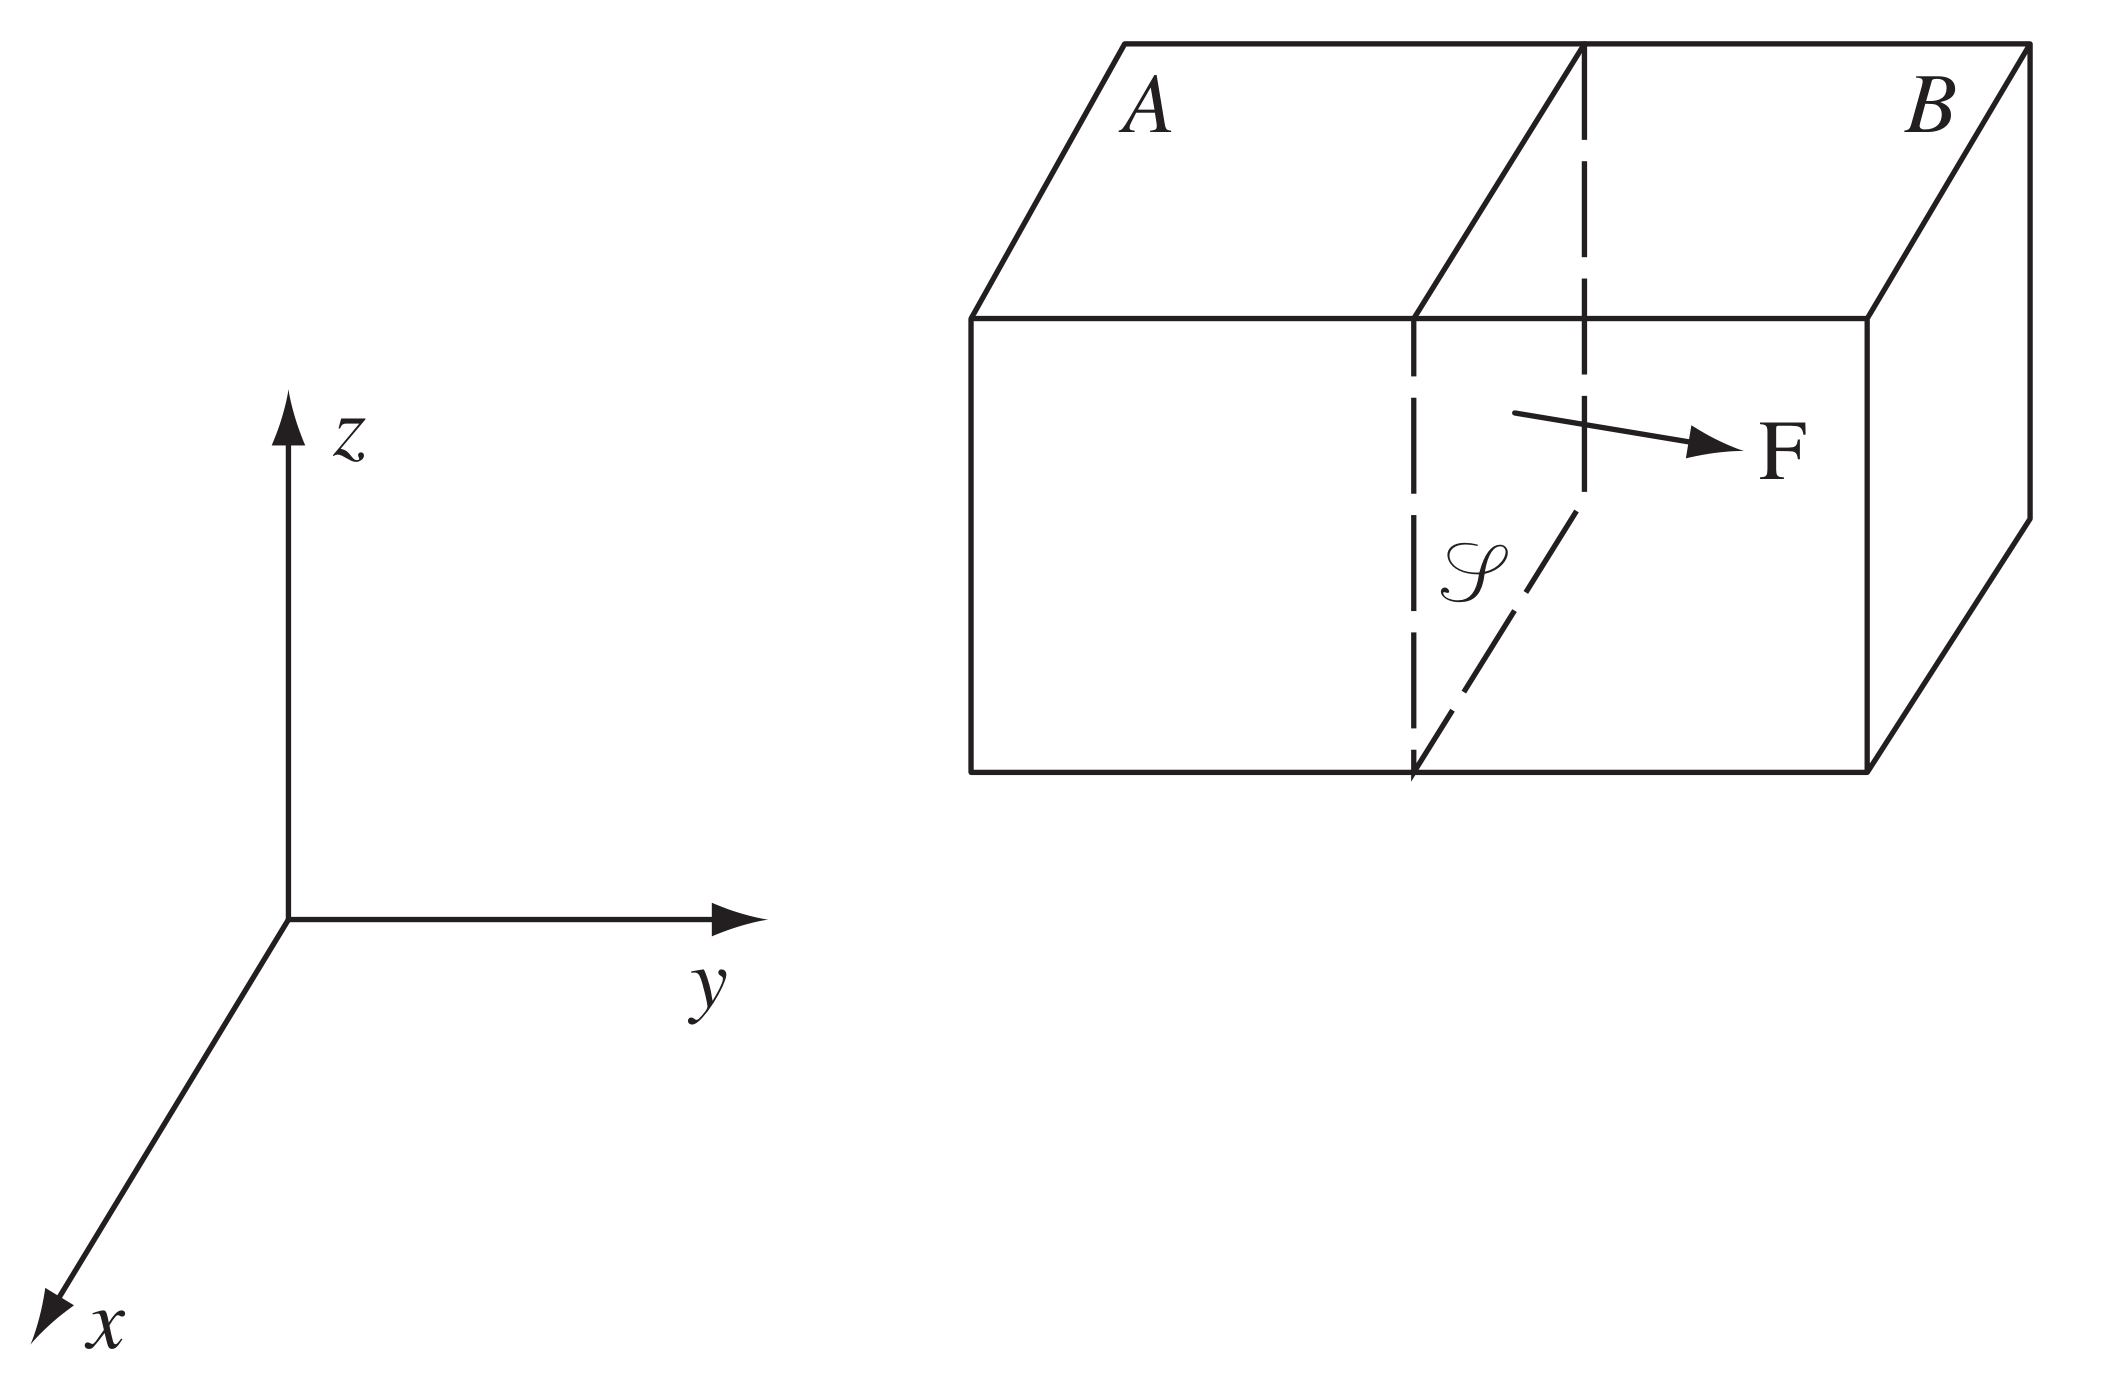
\includegraphics[width=0.6\textwidth]{fig4.6.png}
    \figcaption{\textit{流体元$A$作用于相邻体元$B$的力可能沿任意方向,取决于介质与外力的性质。}}
    \label{fig4.6}
}

图中画出了$A$作用于$B$的力$\bm{F}$(当然,$B$对$A$有等大反向的反作用力)。因为力就是动量的变化率(由于我们在体元速度为零的MCRF中讨论问题,因此牛顿第二定律有效),所以$A$在单位时间内以速度$\bm{F}$向$B$输出动量。当然,取决于相邻体元对它的合外力,体元$B$的动量会发生变化,显然$B$的运动是合外力作用的结果。每个力都向$B$输送动量。从$A$到$B$,穿过界面$\mathscr{S}$,有着速率为$\bm{F}$的动量流量。设$\mathscr{S}$面的面积为$\mathcal{A}$,则通过$\mathscr{S}$面的动量流量为$\bm{F} / \mathcal{A}$。如果$\mathscr{S}$面是等$x^j$面,则流体元$A$的$T^{ij}$等于$F^i / \mathcal{A}$。

$T^{ij}$的物理意义,简单来说,就是相邻流体元之间的力。之前提过,这些力不一定垂直于流体元界面(例如粘性力或其它平行于界面的、为流体提供刚性的力)。如果力\textbf{垂直于}界面,则除非$i = j$,否则$T^{ij} = 0$。(想明白这个结论,后面要用)

\subsection*{MCRF中$T^{\alpha \beta}$的对称性}
现在证明$\mathbf{T}$是对称张量。为此只需要证明它在某一坐标系的分量是对称的,这意味着对任意$\tilde{r}, \tilde{q}$,都有$\mathbf{T} (\tilde{r}, \tilde{q}) = \mathbf{T} (\tilde{q}, \tilde{r})$,也就是说任意坐标系的分量都对称。最简单的坐标系是MCRF。

{
        \centering
        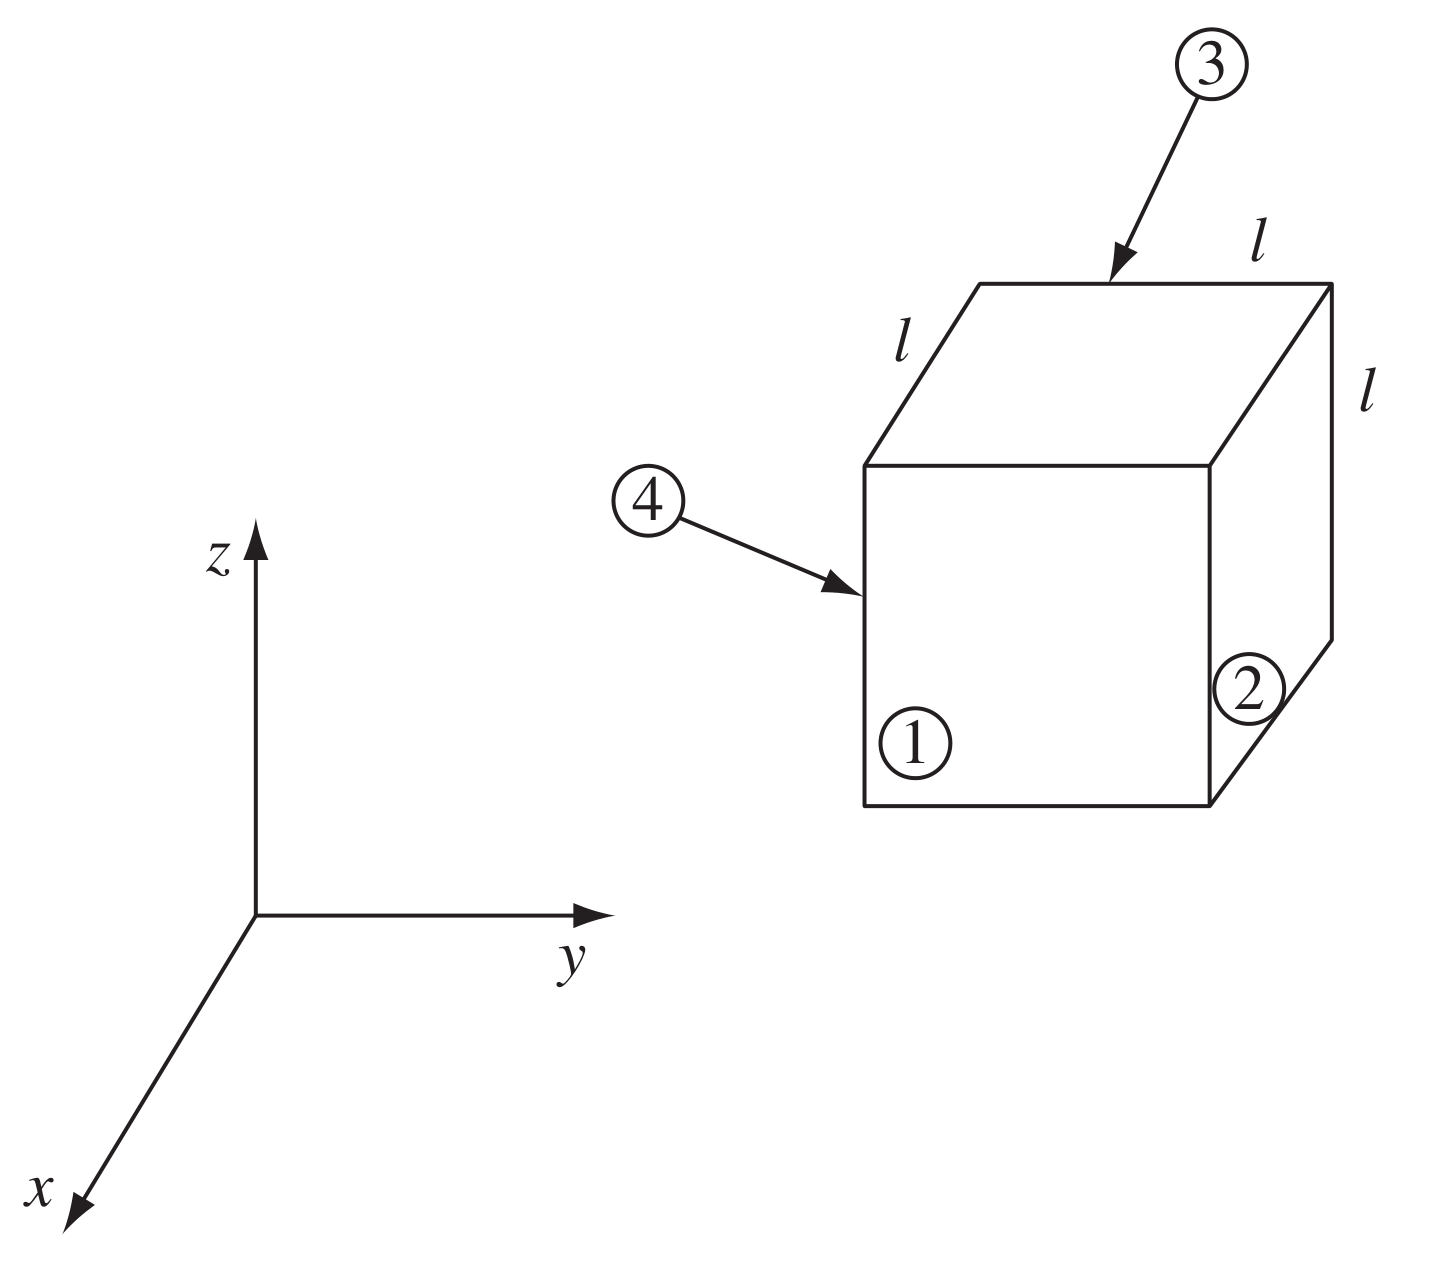
\includegraphics[width=0.6\textwidth]{fig4.7.png}
        \figcaption{\textit{一个流体元。}}
        \label{fig4.7}
}

\begin{enumerate}
    \item $T^{ij}$的对称性。 考虑图\ref{fig4.7},其中画出了边长为$\ell$的立方体流体元。它对与表面(1)(一个$x = \text{constant}$的表面)相邻的体元施加的力等于$F^i_1 = T^{ix} \ell^2$,其中因子$\ell^2$是接触面的面积,由于$\bm{F}$不一定垂直于接触面,因此$i$有$1, 2, 3$三种取值。类似地,该体元通过表面(2)对相邻体元施加的力等于$F_2^i = T^{iy} \ell^2$。(之后会取极限$\ell \to 0$,因此记住流体元很小。)该体元也会对$-x$方向的体元施力,记作$F_3^i$。同理,$F_4^i$是对$-y$方向的力。这个流体元\textbf{所受的}力分别是$-F_1^i, -F_2^i$,等等。

    第一,$F_3^i \approx -F_1^i$,因为体元所受的合力应该随着$\ell \to 0$而趋于零(否则$\ell \to 0$的小质点会有无穷大的加速度)。第二,考虑过体元中心、与$z$轴平行的转轴,计算体元关于该轴的力矩。作用于流体上下表面的力对该力矩无贡献,它们可以忽略。$-\bm{F}_1$对应的力矩为$-(\bm{r} \times \bm{F}_1)^z = -x F_1^y = -\frac{1}{2}\ell T^{yx} \ell^2$,其中将力的作用点近似视为界面中心,$\bm{r} \to (\ell/2, 0, 0)$(注意在那里$y = 0$)。$-\bm{F}_3$对应的力矩\textbf{同样}是$-\frac{1}{2} \ell^3 T^{yx}$。$-\bm{F}_2$的力矩是$-(\bm{r} \times \bm{F}_2)^z = +yF_2^x = \frac{1}{2} \ell T^{xy} \ell^2$. 同理,$-\bm{F}_4$的力矩是$\frac{1}{2} \ell^3 T^{xy}$。因此,总力矩为
    \begin{equation}
        \tau_z = \ell^3 (T^{xy} - T^{yx}).
    \label{equ4.27}
    \end{equation}
    流体元关于$z$轴的转动惯量正比于其质量乘以$\ell^2$,即:
    \[
        I = \alpha \rho \ell^5,
    \]
    其中$\alpha$是某个常数,$\rho$是密度(这里无论是总能量还是静质量都无所谓)。因此角加速度为
    \begin{equation}
        \ddot{\theta} = \frac{\tau}{I} = \frac{T^{xy} - T^{yx}}{\alpha \rho \ell^2}.
    \label{equ4.28}
    \end{equation}
    因为$\alpha$是常数,$\rho$、$T^{xy}\text{与}T^{yx}$与体元的大小无关,所以在$\ell \to 0$的极限下,为了避免无穷大的角加速度,必须
    \[
        T^{xy} = T^{yx}.
    \]
    因此,根据流体元没有绕内部流体旋转、越小的流体并非旋转越快,我们得出结论,应力总是\textbf{对称的}:
    \begin{equation}    
        T^{ij} = T^{ji}.
    \label{equ4.29}
    \end{equation}  
    推导过程并未涉及物质的特殊性质,因此该结论对固体、流体都适用。在狭义相对论中,牛顿理论也能用,牛顿理论中$T^{ij}$是三维$\binom{2}{0}$张量——应力张量的分量,材料工程师对它很熟悉,它的名字保留作为相对论推广量$\mathbf{T}$的一部分。
    \item 动量密度等于能量流的证明。这比上一条简单多了。能量流是能量密度乘以能量流动的速率,由于能量与质量相同,因此能量流等于质量密度乘以它流动的速率;换句话说,就是动量密度,因此$T^{0i} = T^{i0}$.    
\end{enumerate}


\subsection*{能量-动量守恒}
由于$\mathbf{T}$表示流体的能量、动量,因此可以用它表示能量动量守恒定律,实际上相应的形式超级简单。考虑图\ref{fig4.8}中的管状体元,只考虑其横截面(图中省略了$z$轴)。

{
    \centering
    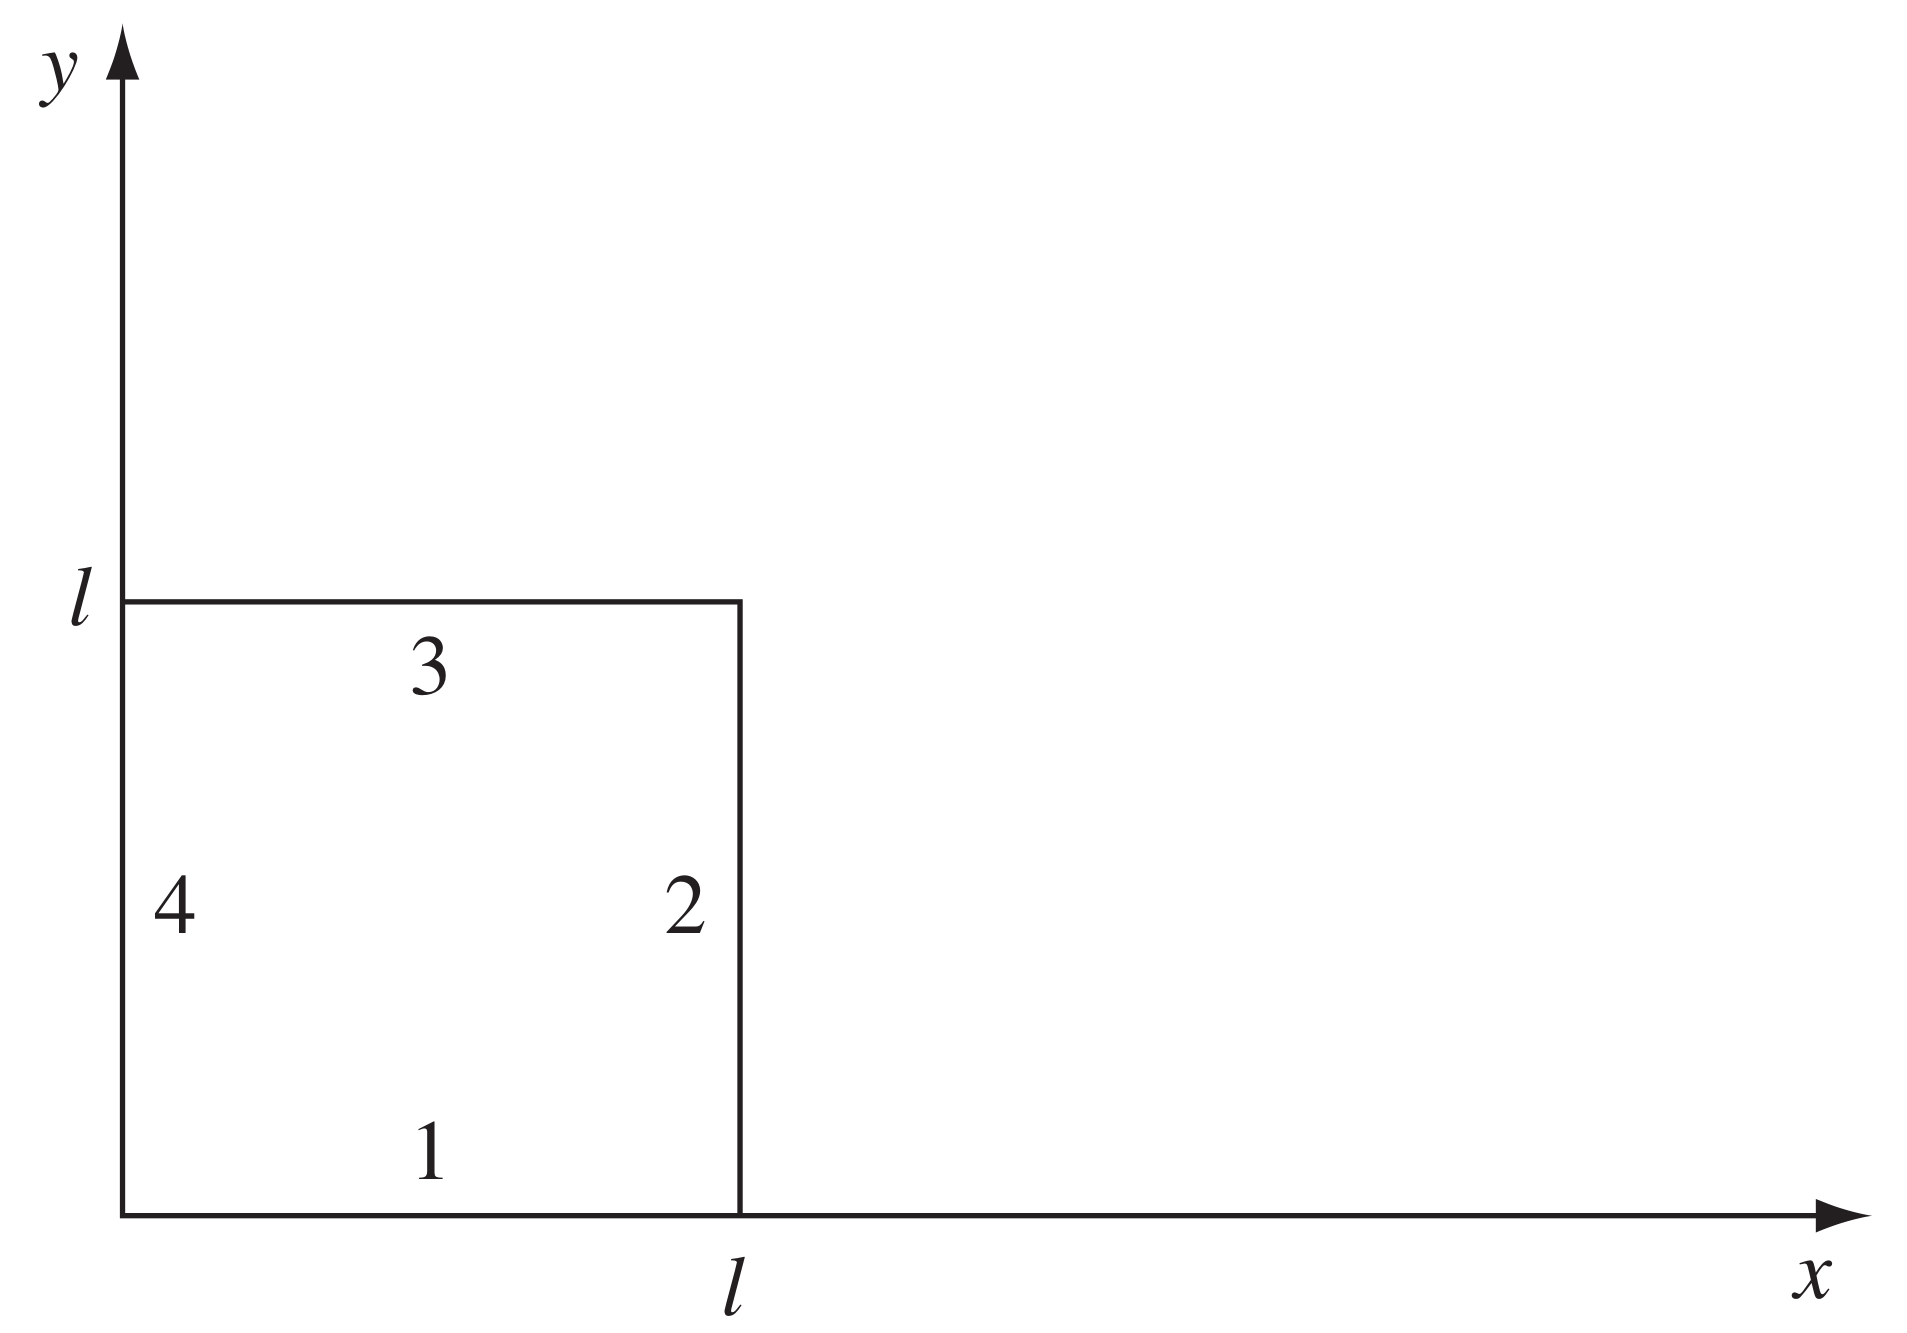
\includegraphics[width=0.6\textwidth]{fig4.8.png}
    \figcaption{\textit{一个管状流体元的$z = \text{constant}$横截面。}}
    \label{fig4.8}
}

能量可以从体元的各个表面流进流出。能量通过表面(4)流入体元的速率为$\ell^2 T^{0x} (x = 0)$;通过表面(2)流入体元的速率为$-\ell^2 T^{0x} (x = a)$,注意其中的负号,因为$T^{0x}$表示能量沿正$x$方向的流动,它在(2)处取值的方向为流出体元。同理,从$y$方向流入体元的能量为$\ell^2 T^{0y} (y = 0) - \ell^2 T^{0y} (y = \ell)$。根据能量守恒,它们之和等于流体元能量的增长率$\partial(T^{00} \ell^3) / \partial t$,由此可得
\begin{align}
    \frac{\partial}{\partial t} (\ell^3 T^{00}) = \ell^2 \Big[& T^{0x}|_{x = 0} - T^{0x}|_{x = \ell} \notag \\
    & + T^{0y}|_{y = 0} - T^{0y}|_{y = \ell} + T^{0z}|_{z = 0} - T^{0z}|_{z = \ell} \Big]. \label{equ4.30}
\end{align}
两边除以$\ell^3$并取极限$\ell \to 0$,并注意到
\begin{equation}
\lim_{\ell \to 0} \dfrac{T^{0x}|_{x = 0} - T^{0x}|_{x = \ell}}{\ell} \equiv -\frac{\partial}{\partial x} T^{0x},
\label{equ4.32}
\end{equation}
于是\eqref{equ4.30}式化为:
\begin{equation}
    \frac{\partial}{\partial t} T^{00} = -\frac{\partial}{\partial x} T^{0x} - \frac{\partial}{\partial y} T^{0y} - \frac{\partial}{\partial z} T^{0z}.
\label{equ4.31}
\end{equation}

\eqref{equ4.31}式可以写为
\begin{align}
    T\indices{^{00}_{, 0}} &+ T\indices{^{0x}_{,x}} + T\indices{^{0y}_{,y}} + T\indices{^{0z}_{,z}} = 0 \notag \\
\intertext{或者}
    T\indices{^{0\alpha}_{, \alpha}} &= 0. \label{equ4.33}
\end{align}
这就是能量守恒的表达式。

动量守恒的情形同理。利用相似的推导过程,可以证明$T\indices{^{i \alpha}_{, \alpha}} = 0$,因此一般的守恒定律可以表述为
\begin{shaded}
\begin{equation}
    T\indices{^{\alpha \beta}_{, \beta}} = 0.
\label{equ4.34}
\end{equation}
\end{shaded}
这对SR中的任何系统都成立。注意,上式就是四维散度,因而与高斯定理(守恒律的积分形式)有关,后面会进行相关讨论。

\subsection*{粒子守恒}
在流体流动的过程中,流体元的粒子数可能会改变,但是流体总体的粒子数不变。在图\ref{fig4.8}中,流体元当中粒子数的变化是由于粒子从边界面流入流出引起的,变化率等于流入或流出的净流量。这种粒子数守恒可以通过与\eqref{equ4.34}式类似的方式推导出来,这里直接给出结果:
\[
    \frac{\partial}{\partial t} N^0 = -\frac{\partial}{\partial x} N^x - \frac{\partial}{\partial y} N^y - \frac{\partial}{\partial z} N^z,
\]
或者写为
\begin{shaded}
\begin{equation}
    N\indices{^\alpha_{, \alpha}}  = (n U^\alpha)_{, \alpha} = 0.
\label{equ4.35}
\end{equation}
\end{shaded}
我们只考虑这种服从粒子数守恒的流体。这是个很弱的限制,因为粒子数密度$n$几乎总可以取为重子的,重子绝大部分情况下守恒。

对于不熟悉高能物理的人,“重子(baryon)”的概念比较陌生,它是物理学中一类大质量粒子的统称,最常见的重子是中子和质子。其它重子不稳定,在日常物理学的地位不如前两者重要,但是它们会衰变成质子和中子,保证了重子数守恒,但不能保证静质量、特定种类的重子数。尽管理论物理学家认为重子数可能不守恒——例如,强、弱和电磁相互作用的“大统一理论”认为质子具有有限长的寿命,黑洞的坍缩与之后的蒸发(见\ref{chap11}章)不满足重子数守恒——但是这些现象目前并未观测到,而且在大部分情况下都不重要。


\section{理想流体}
\label{sec4.6}

\section{对于广义相对论的重要性}
\label{sec4.7}

\section{高斯定律}
\label{sec4.8}

\section{扩展阅读}
\label{sec4.9}

\section{习题}
\label{sec4.10}